\PassOptionsToPackage{full}{textcomp}
\documentclass[a4paper, nobib]{tufte-book}

% fonts
\usepackage[p, osf]{ETbb}
\usepackage[scaled=.95,type1]{cabin}
\usepackage[libertine, vvarbb]{newtxmath}

% misc
\usepackage{booktabs}
\usepackage{amsmath}
\usepackage{capt-of}
\usepackage{bm}

\usepackage{tikz}
\usetikzlibrary{calc}
\usetikzlibrary{fit}
\usetikzlibrary{positioning}
\usetikzlibrary{matrix}
\usetikzlibrary{arrows,shapes}
\usetikzlibrary{arrows.meta} 
\usetikzlibrary{graphs} 
\usetikzlibrary{trees} 
\usetikzlibrary{quotes} 
\usetikzlibrary{decorations.text}
\usetikzlibrary{decorations.markings}

\renewcommand{\vec}[1]{\bm{#1}}
\def\y#1#2{\hat{\lambda}_{#1#2}}
\def\yy#1#2{1\!-\!\y{#1}{#2}}

\definecolor{color0}{HTML}{001118}
\definecolor{color1}{HTML}{005e72}
\definecolor{color2}{HTML}{0a9395}
\definecolor{color3}{HTML}{93d1bc}
\definecolor{color4}{HTML}{e8d8a5}
\definecolor{color5}{HTML}{ed9a00}
\definecolor{color6}{HTML}{ca6702}
\definecolor{color7}{HTML}{ba3d02}
\definecolor{color8}{HTML}{ae1f11}
\definecolor{color9}{HTML}{9a2126}


\begin{document}

\listoffigures

\begin{figure}
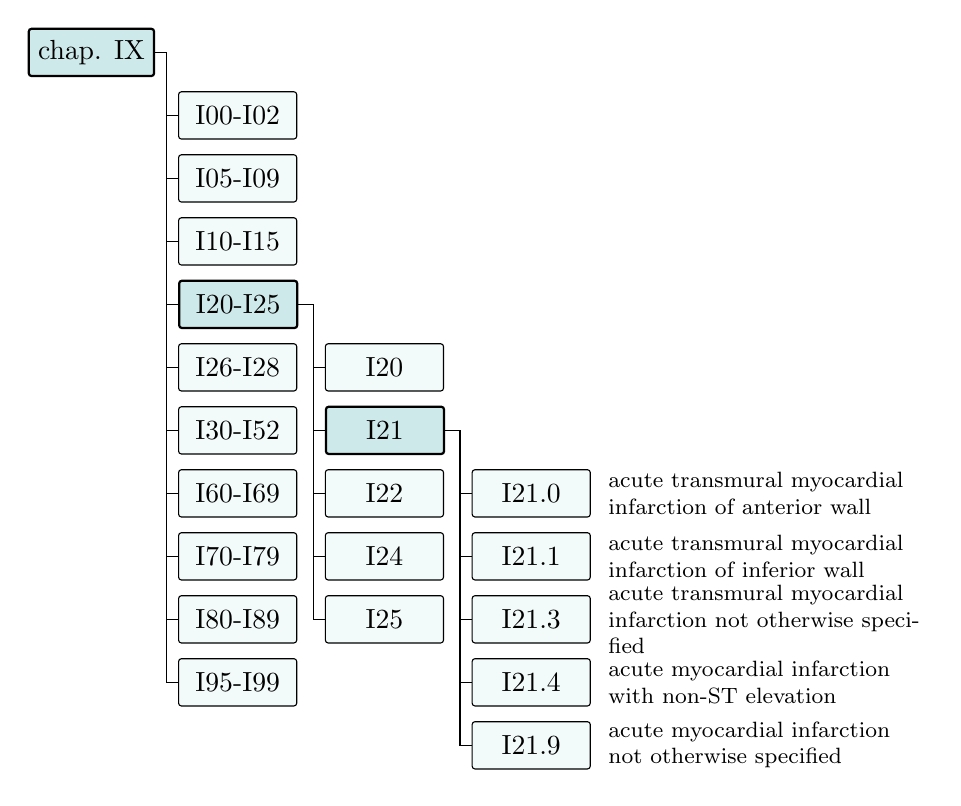
\begin{tikzpicture}[
    every node/.append style = {
        draw, anchor = west, 
        minimum width=1.5cm, 
        minimum height=6mm,
        font=\tlfstyle,
        rounded corners=1pt,
        fill=color2!5
    },
    sel/.style = {fill=color2!20, draw=black, thick},
    txt/.style = {fill=none, draw=none, font=\footnotesize, text width=4.0cm},
    grow via three points={
        one child    at (1.1, -0.8) and 
        two children at (1.1, -0.8) 
                    and (1.1, -1.6)
    },
    edge from parent path={
        (\tikzparentnode.east) 
        -| ([xshift=-4.2]\tikzchildnode.west)
        |- (\tikzchildnode.west)
    }]

    \node[sel] {chap. IX}
        child {node {I00-I02}}
        child {node {I05-I09}}
        child {node {I10-I15}}
        child {node[sel] {I20-I25}
            child {node (i20) {I20}}
            child {node [sel] (i21) {I21}
                child {node (1) {I21.0}}
                child {node (2) {I21.1}}
                child {node (3) {I21.3}}
                child {node (4) {I21.4}}
                child {node (5) {I21.9}}
            }
            child {node {I22}}
            child {node {I24}}
            child {node {I25}}
        }
        child {node {I26-I28}}
        child {node {I30-I52}}
        child {node {I60-I69}}
        child {node {I70-I79}}
        child {node {I80-I89}}
        child {node {I95-I99}}
    ;
    \node [txt, right=1mm of 1] {acute transmural myocardial infarction of anterior wall};
    \node [txt, right=1mm of 2] {acute transmural myocardial infarction of inferior wall};
    \node [txt, right=1mm of 3] {acute transmural myocardial infarction not otherwise specified};
    \node [txt, right=1mm of 4] {acute myocardial infarction with non-ST elevation};
    \node [txt, right=1mm of 5] {acute myocardial infarction not otherwise specified};
\end{tikzpicture}
\caption{This is my caption}
\end{figure}
\end{document}

